\documentclass[12pt,a4paper]{article}
\usepackage[margin=2.4cm]{geometry}
\usepackage{fontspec,polyglossia}
\setmainlanguage[numerals=maghrib]{arabic}
\setotherlanguage{english}
% Shared Arabic font families for XeLaTeX (Amiri with explicit bold/italic).
\defaultfontfeatures{Ligatures=TeX}
\newfontfamily\arabicfont[
  Script=Arabic,
  Language=Arabic,
  Scale=1.05,
  BoldFont={Amiri Bold},
  ItalicFont={Amiri Italic},
  BoldItalicFont={Amiri Bold Italic}
]{Amiri}
\newfontfamily\arabicfontsf[
  Script=Arabic,
  Language=Arabic,
  Scale=1.05,
  BoldFont={Amiri Bold},
  ItalicFont={Amiri Italic},
  BoldItalicFont={Amiri Bold Italic}
]{Amiri}
\newfontfamily\arabicfonttt[
  Script=Arabic,
  Language=Arabic,
  Scale=0.95,
  BoldFont={Amiri Bold}
]{Amiri}

\usepackage{amsmath,amssymb,booktabs,graphicx,hyperref}
\graphicspath{{../../figures/}}
\title{\textbf{نتائج تجريبية لعائلة DA-SFCN}\\
\large هروب السرج وتعقيد الأوراكل ومعايير الامتدادات\\
\large (تقرير التنفيذ المرجعي)}
\author{مجموعة التحسين العددي --- DA-SFCN}
\date{سبتمبر 2026}
\begin{document}
\maketitle

\begin{abstract}
نورد تجارب \textenglish{CPU} قابلة لإعادة الإنتاج لخوارزمية نيوتن التكعيبي
الخالي من السرج ذي البعد الديناميكي \textenglish{(DA-SFCN)} وامتداداتها، عبر
الحزمة المفتوحة \texttt{dasfcn}. على سرج رباعي غير محدد، تفلت
\textenglish{DA-SFCN} ونيوتن الخالي من السرج في \emph{كل} المحاولات متعددة
البذور، بينما لا يفلت انحدار التدرّج في أيٍّ منها. وعلى مجموعة مسائل تحليلية
وأسلوب تعلّم آلة نجدول معايير التدرّج وقيم الهدف وعدد جداءات الهيسيان--متجه
\textenglish{(HVP)}. ويطابق \textenglish{LK-Newton} الدقة غالبًا بجزء من تكلفة
الجداءات. الأرقام مأخوذة من
\texttt{results/summary.json} و\texttt{results/repro\_smoke.json}.
\end{abstract}

\section{الإعداد}
الحزمة \texttt{dasfcn} (رخصة \textenglish{MIT}) وواجهة
\texttt{minimize} وسكربت \texttt{scripts/repro\_smoke.py}.
المقياس الأساسي هو عدد \textenglish{HVP} لا زمن الجدار وحده، والتجارب مضبوطة
للابتوب: $n\le 80$ في المجموعة الرئيسية و$n=40$ في اختبار البذور، دون ضبط
نماذج لغة.

\section{هروب السرج متعدد البذور}
المسألة: \texttt{QuadraticSaddle} ببعد 40 وست قيم ذاتية سالبة، ثمانية
بدءات عشوائية، نجاح إذا $\|\nabla f\|<10^{-3}$ و$f<0.05$ خلال 40 تكرارًا.

\begin{table}[h]
\centering
\caption{نجاح الهروب في 8 بذور ($n=40$).}
\begin{tabular}{@{}lrrr@{}}
\toprule
الطريقة & النجاحات & النسبة & متوسط \textenglish{HVP} \\
\midrule
تدرّج & 0/8 & 0\% & --- \\
\textenglish{L-BFGS} & 7/8 & 87.5\% & 0 \\
\textenglish{SFN} & 8/8 & 100\% & 235.1 \\
\textenglish{DA-SFCN} & 8/8 & 100\% & 256.1 \\
\bottomrule
\end{tabular}
\end{table}

\begin{figure}[h]
\centering
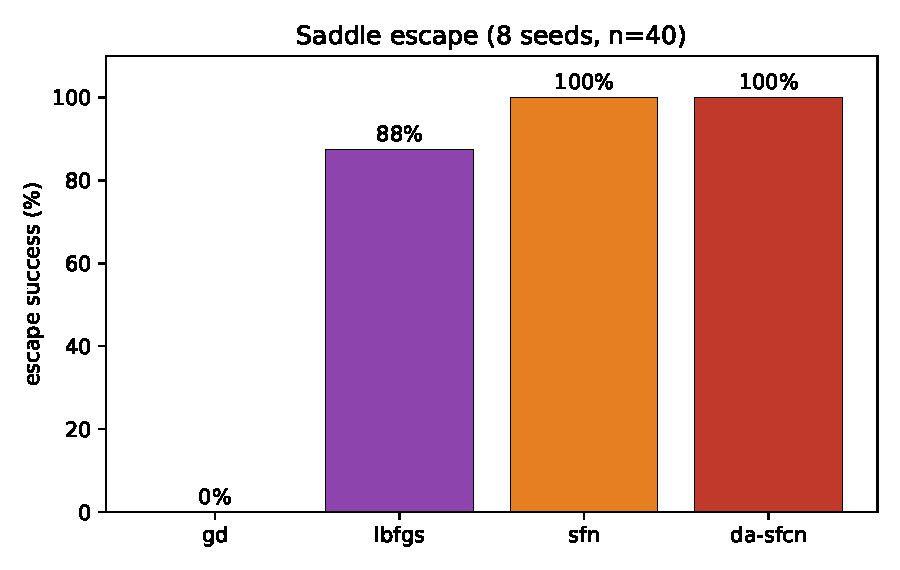
\includegraphics[width=0.72\textwidth]{fig_repro_success.pdf}
\caption{نسب نجاح الهروب من سكربت إعادة الإنتاج.}
\end{figure}

\begin{figure}[h]
\centering
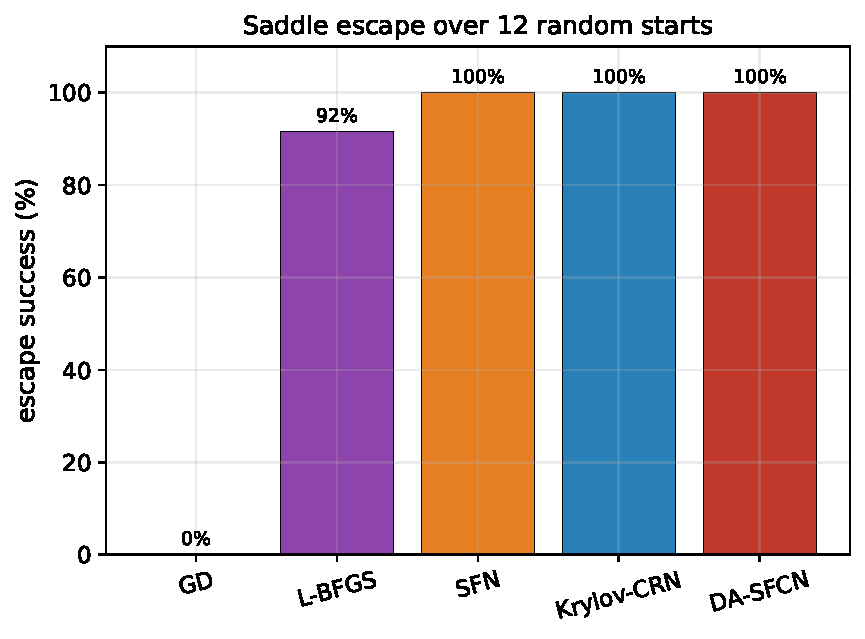
\includegraphics[width=0.48\textwidth]{fig_success.pdf}
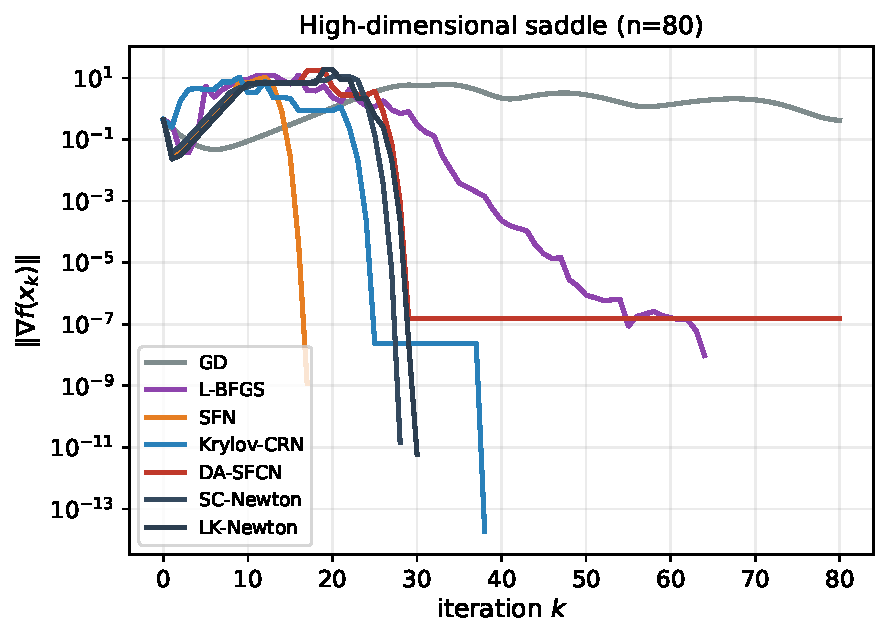
\includegraphics[width=0.48\textwidth]{fig_saddle_highdim.pdf}
\caption{يسار: دراسة سابقة بـ 12 بدءًا. يمين: معيار التدرّج على سرج $n=80$.}
\end{figure}

\textbf{الخلاصة.} انحدار التدرّج يفشل تحت هذه الميزانية.
\textenglish{L-BFGS} قوي غير مكتمل. طرائق الانحناء السالب / كريلوف التكعيبي
تنجح في كل تجارب الـ smoke.

\section{المجموعة الرئيسية}
\subsection{سرج عالي البعد ($n=80$)}
\begin{table}[h]
\centering
\caption{سرج تربيعي-رباعي، $n=80$.}
\begin{tabular}{@{}lrrr@{}}
\toprule
الطريقة & التكرارات & $\|\nabla f\|$ النهائي & \textenglish{HVP} \\
\midrule
تدرّج & 80 & $4.19\times10^{-1}$ & 0 \\
\textenglish{L-BFGS} & 64 & $9.63\times10^{-9}$ & 0 \\
\textenglish{SFN} & 17 & $1.16\times10^{-9}$ & 204 \\
\textenglish{Krylov-CRN} & 38 & $1.82\times10^{-14}$ & 456 \\
\textenglish{DA-SFCN} & 80 & $1.53\times10^{-7}$ & 1219 \\
\textenglish{SC-Newton} & 28 & $1.42\times10^{-11}$ & 413 \\
\textenglish{LK-Newton} & 30 & $5.87\times10^{-12}$ & \textbf{158} \\
\bottomrule
\end{tabular}
\end{table}
كل طرائق الرتبة الثانية تبلغ $f^\star\approx -89.58$.
\textenglish{LK-Newton} الأرخص بالجداءات مع دقة مكافئة.

\subsection{لوجستي غير محدب}
\begin{table}[h]
\centering
\caption{لوجستي غير محدب ($N=350$, $n=50$).}
\begin{tabular}{@{}lrrr@{}}
\toprule
الطريقة & التكرارات & $\|\nabla f\|$ النهائي & \textenglish{HVP} \\
\midrule
تدرّج & 39 & $7.36\times10^{-9}$ & 0 \\
\textenglish{L-BFGS} & 9 & $2.09\times10^{-9}$ & 0 \\
\textenglish{SSCN-coord} & 70 & $1.20\times10^{-8}$ & 700 \\
\textenglish{Krylov-CRN} & 5 & $1.35\times10^{-10}$ & 50 \\
\textenglish{DA-SFCN} & 6 & $4.85\times10^{-13}$ & 66 \\
\textenglish{VR-DA-SFCN} & 19 & $4.73\times10^{-14}$ & 244 \\
\bottomrule
\end{tabular}
\end{table}

\begin{figure}[h]
\centering
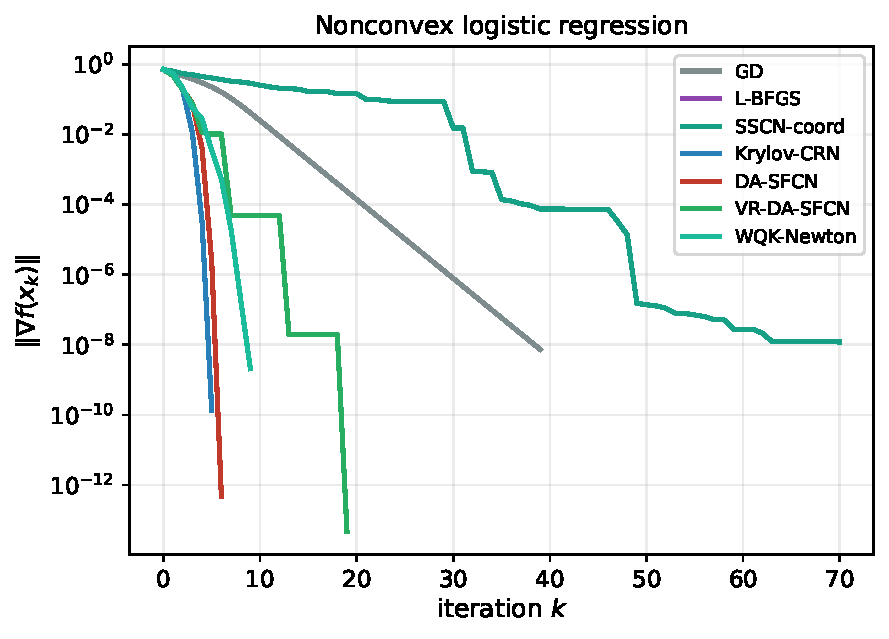
\includegraphics[width=0.48\textwidth]{fig_logistic.pdf}
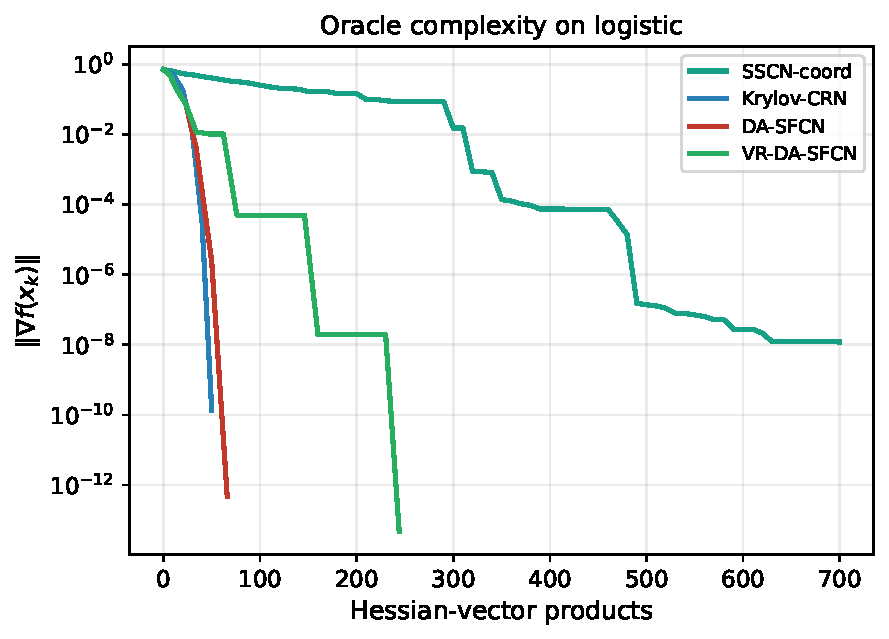
\includegraphics[width=0.48\textwidth]{fig_logistic_hvp.pdf}
\caption{اللوجستي غير المحدب: التدرّج مقابل التكرار (يسار) ومقابل \textenglish{HVP} (يمين).}
\end{figure}

\subsection{تحليل مصفوفات ووعاء تربيعي}
على تحليل المصفوفات تهبط $f$ إلى $4.95\times10^{-28}$ في 19 خطوة
(130 \textenglish{HVP}). وفي وعاء تربيعي محدب قوي تكفي تكرارتان لبلوغ
$\|\nabla f\|\approx10^{-10}$ (27 جداءً)، مقابل $\approx10^{-2}$ بعد 40
خطوة تدرّج.

\begin{figure}[h]
\centering
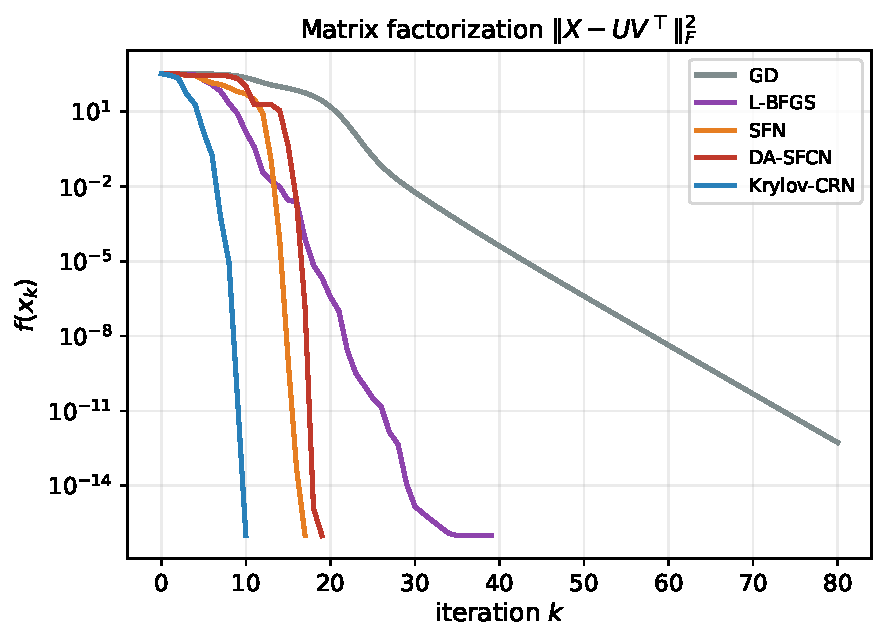
\includegraphics[width=0.48\textwidth]{fig_factor.pdf}
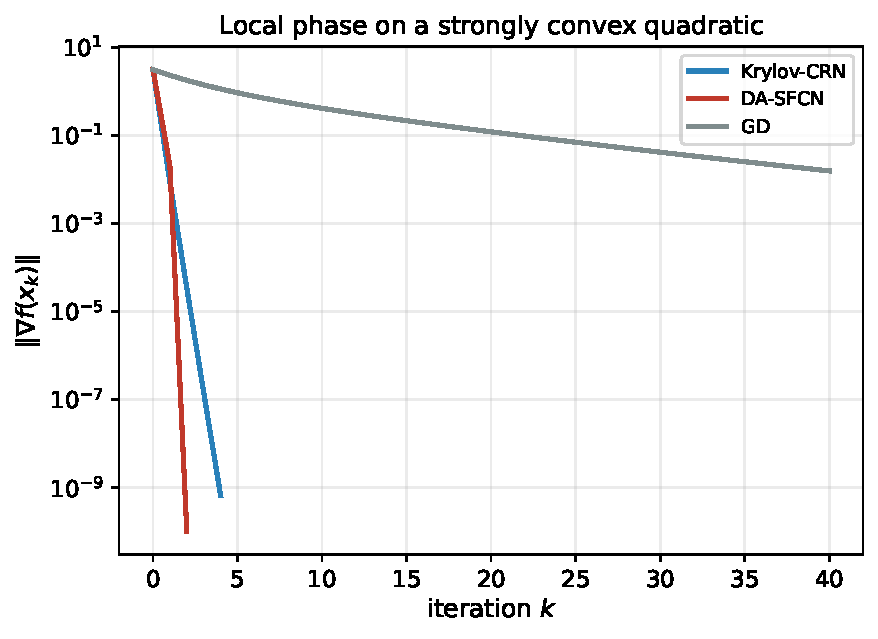
\includegraphics[width=0.48\textwidth]{fig_local.pdf}
\caption{تحليل المصفوفات (يسار) والوعاء التربيعي المحلي (يمين).}
\end{figure}

\subsection{مجموع منتهٍ / فيدرالي / روزنبروك}
\textenglish{DA-SFCN} الكامل: 8 تكرارات و82 جداءً
($\|\nabla f\|\approx7.2\times10^{-11}$)؛ و\textenglish{Fed-DA-SFCN}
يستقر عند $\sim4.3\times10^{-4}$ كما يتوقع عدم التجانس؛ وروزنبروك يبقى
اختبار إجهاد يبرّر تهيئة \textenglish{Lanczos}
(\texttt{dasfcn/precond.py}).

\begin{figure}[h]
\centering
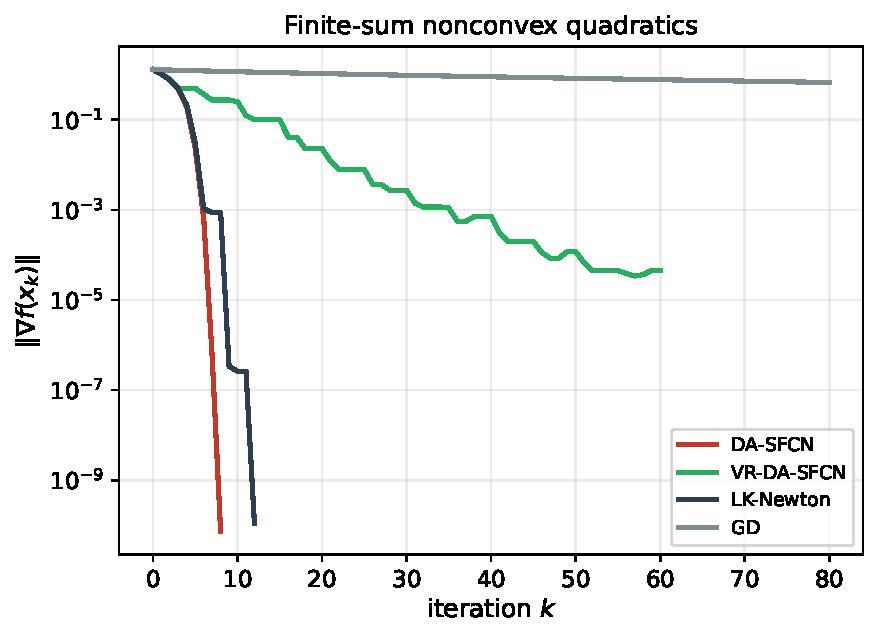
\includegraphics[width=0.32\textwidth]{fig_vr.pdf}
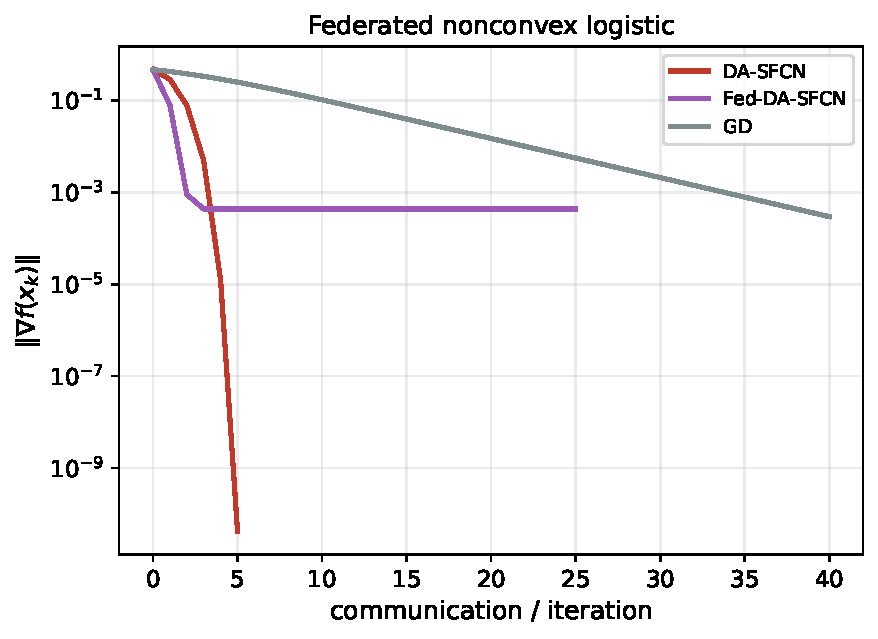
\includegraphics[width=0.32\textwidth]{fig_fed.pdf}
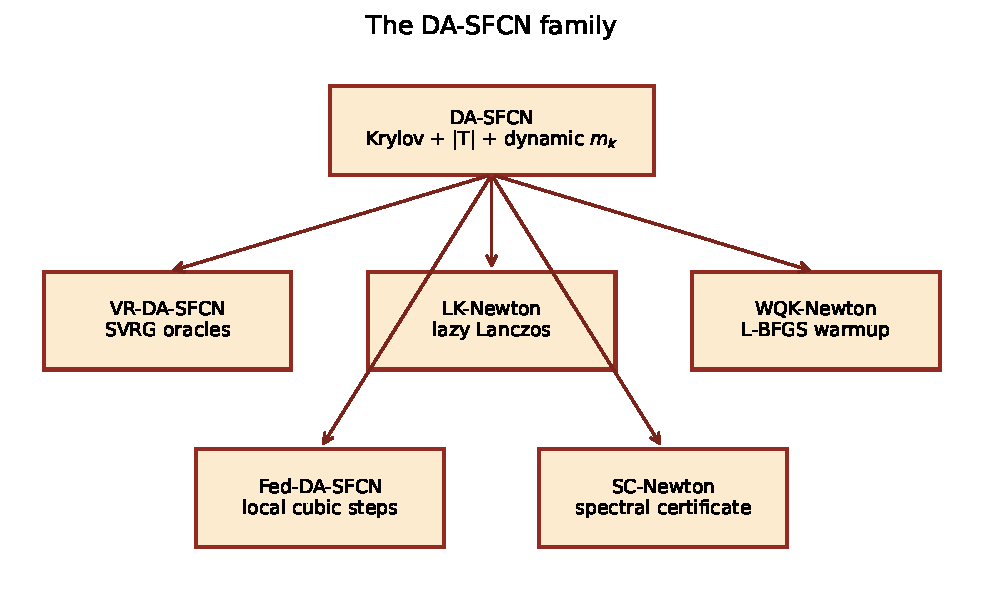
\includegraphics[width=0.32\textwidth]{fig_family.pdf}
\caption{مجموع منتهٍ (يسار)، فيدرالي (وسط)، نظرة عائلية (يمين).}
\end{figure}

\section{التحقق البرمجي}
تسعة اختبارات وحدة ناجحة على \textenglish{CPU}. وفي smoke اللوجستي:
$\|\nabla f\|\approx7.7\times10^{-13}$ بعد 43 جداءً.

\section{الخاتمة}
\begin{enumerate}
\item \textenglish{DA-SFCN} (و\textenglish{SFN}) تفلت بموثوقية من سروج تحليلية يفشل فيها التدرّج.
\item اقتصاد \textenglish{HVP} يرجّح \textenglish{LK-Newton} و\textenglish{SC-Newton} عند الإعادة/الشهادة.
\item الحزمة تجعل الادعاءات قابلة لإعادة الإنتاج على لابتوب:
  \texttt{pytest} و\texttt{scripts/repro\_smoke.py}.
\item فجوات المرجع العالمي الأوسع (LIBSVM، شبكات، LLM مقابل Sophia) مؤجَّلة
  عمدًا لعتاد أقوى كما في \texttt{docs/OPTIMIZER.md}.
\end{enumerate}

\begin{english}
\begin{thebibliography}{6}
\bibitem{nesterov2006} Nesterov, Polyak. \textit{Math.\ Program.}, 2006.
\bibitem{cartis2011} Cartis, Gould, Toint. ARC. \textit{Math.\ Program.}, 2011.
\bibitem{jiang2024} Jiang et al. Krylov CRN. \textit{AISTATS}, 2024.
\bibitem{dauphin2014} Dauphin et al. \textit{NeurIPS}, 2014.
\bibitem{repo} \url{https://github.com/jameljoni1994-ENG/DA-SFCN}, 2026.
\end{thebibliography}
\end{english}
\end{document}
